ran the tests 
starting parallel test 1
\def \CILKserialbaseline {4.8}
\def \CILKblocksize {64}
\def \CILKnumtrials {5}
\def \CILKinputsize {1048576}
\def \CILKtable {
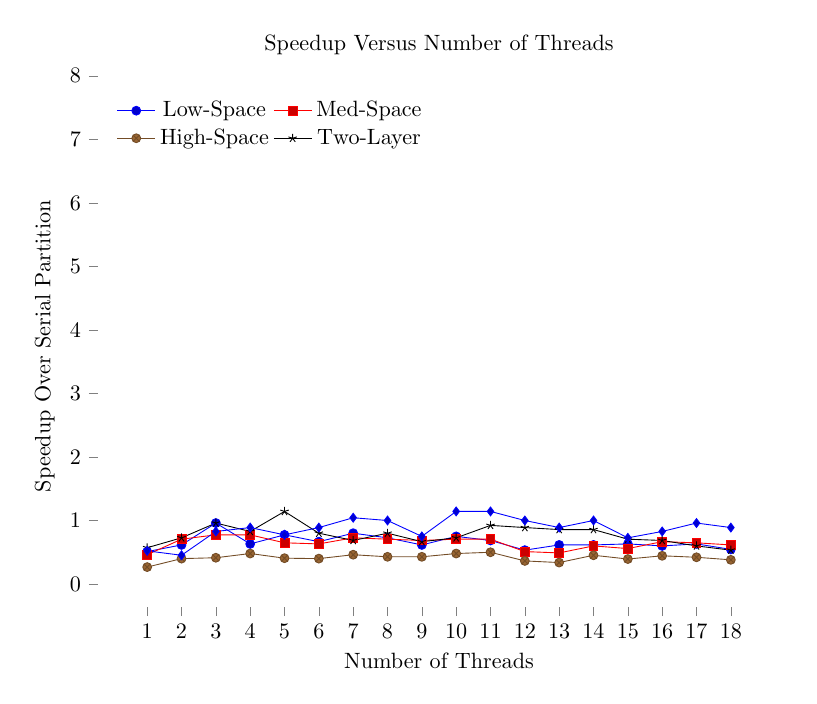
\begin{tikzpicture}[scale = .8]
\begin{axis}[
width = 5 in,
height = 4in,
title={Speedup Versus Number of Threads},
xtick pos=left,
ytick pos=left,
legend style={draw=none},
axis line style = { draw = none },
legend pos= north west,
xtick = data,
xlabel={Number of Threads},
ylabel={Speedup Over Serial Partition},
ymax = 8,
legend columns = 2,
scatter/classes=%
{a={mark=o,draw=blue}}]
%% In-Place
\addplot coordinates {( 1, 0.510638) ( 2, 0.615385) ( 3, 0.96) ( 4, 0.631579) ( 5, 0.774194) ( 6, 0.666667) ( 7, 0.8) ( 8, 0.727273) ( 9, 0.615385) ( 10, 0.75) ( 11, 0.685714) ( 12, 0.533333) ( 13, 0.615385) ( 14, 0.615385) ( 15, 0.631579) ( 16, 0.6) ( 17, 0.631579) ( 18, 0.545455) };
%% In-Place Prefix-Sum
\addplot coordinates {( 1, 0.461538) ( 2, 0.705882) ( 3, 0.774194) ( 4, 0.774194) ( 5, 0.648649) ( 6, 0.631579) ( 7, 0.727273) ( 8, 0.705882) ( 9, 0.685714) ( 10, 0.705882) ( 11, 0.705882) ( 12, 0.510638) ( 13, 0.489796) ( 14, 0.6) ( 15, 0.55814) ( 16, 0.666667) ( 17, 0.648649) ( 18, 0.615385) };
%% Out-of-Place
\addplot coordinates {( 1, 0.266667) ( 2, 0.4) ( 3, 0.413793) ( 4, 0.48) ( 5, 0.40678) ( 6, 0.4) ( 7, 0.461538) ( 8, 0.428571) ( 9, 0.428571) ( 10, 0.48) ( 11, 0.5) ( 12, 0.363636) ( 13, 0.338028) ( 14, 0.45283) ( 15, 0.393443) ( 16, 0.444444) ( 17, 0.421053) ( 18, 0.380952) };
%% High-Span
\addplot coordinates {( 1, 0.571429) ( 2, 0.727273) ( 3, 0.96) ( 4, 0.827586) ( 5, 1.14286) ( 6, 0.8) ( 7, 0.685714) ( 8, 0.8) ( 9, 0.666667) ( 10, 0.727273) ( 11, 0.923077) ( 12, 0.888889) ( 13, 0.857143) ( 14, 0.857143) ( 15, 0.705882) ( 16, 0.685714) ( 17, 0.6) ( 18, 0.533333) };
%% Cache-Friendly
\addplot coordinates {( 1, 0.521739) ( 2, 0.45283) ( 3, 0.827586) ( 4, 0.888889) ( 5, 0.774194) ( 6, 0.888889) ( 7, 1.04348) ( 8, 1) ( 9, 0.75) ( 10, 1.14286) ( 11, 1.14286) ( 12, 1) ( 13, 0.888889) ( 14, 1) ( 15, 0.727273) ( 16, 0.827586) ( 17, 0.96) ( 18, 0.888889) };
\legend{Low-Space, Med-Space, High-Space, Two-Layer}
\end{axis}
\end{tikzpicture}
}
starting parallel test 2
\def \cilktwoblocksizetwo {64}
\def \cilktwonumtrialstwo {5}
\def \cilktwonumcorestwo {18}
\def \cilktwoinputsizetwo {1048576}
\def \cilktwotabletwo {
\begin{tikzpicture}[scale = .8]
\begin{axis}[
width = 5 in,
height = 4in,
title={Speedup Versus Input Size},
xtick pos=left,
ytick pos=left,
legend style={draw=none},
axis line style = { draw = none },
legend pos= north west,
xtick = data,
xlabel={Log Input Size},
ylabel={Speedup Over Serial Partition},
ymax = 5,
ymin = 0,
legend columns = 2,
scatter/classes=%
{a={mark=o,draw=blue}}]
%% Serial Baseline
%% baselines in ms: \addplot coordinates {};
%% In-Place
\addplot coordinates {};
%% In-Place Prefix-Sum
\addplot coordinates {};
%% Out-of-Place
\addplot coordinates {};
%% High-Span
\addplot coordinates {};
%% Cache-Friendly
\addplot coordinates {};
\legend{Low-Space, Med-Space, High-Space, Two-Layer}
\end{axis}
\end{tikzpicture}
}
\def \CILKsortblocksize {64}
\def \CILKsortnumtrials {5}
\def \CILKsortmaxinputsize {1048576}
\def \CILKsorttable {
\begin{tikzpicture}[scale = .8]
\begin{axis}[
width = 5 in,
height = 4in,
title={Speedup Versus Number of Threads},
xtick pos=left,
ytick pos=left,
legend style={draw=none},
axis line style = { draw = none },
legend pos= north west,
xtick = data,
xlabel={Number of Threads},
ylabel={Speedup Over Serial Partition},
ymax = 6,
legend columns = 2,
scatter/classes=%
{a={mark=o,draw=blue}}]
\legend{ Low-Space 24, Low-Space 26, Low-Space 28, Two-Layer 24, Two-Layer 26, Two-Layer 28}
\end{axis}
\end{tikzpicture}
}
